%%%%%%%%%% MECHANIC %%%%%%%%%%%%%%%%%%%%%%%%%%%%%%%%%%%%%%%%%%%%%%%%%%%%%%%
\subsection{Assebly}

This section will cover how to put together all the individual pieces that compose the robot in a step-by-step guide.\\


The first part to be assembled is the one with the greatest number of pieces, the gripper. This was designed by \textbf{http://www.thingiverse.com/thing:5735}, and is used because of its parallel way of closing, which guarantees a good grip at any degree of aperture. In order to build it, the corresponding lettered holes simply have to be connected, as shown in Figure \ref{ass1}. These must be fastened together with M3x25mm screws, except for hole ``A" and the wrist servo, which are fastened with the bolts included with the servos.\\

	\begin{figure}[H]
			\centering
			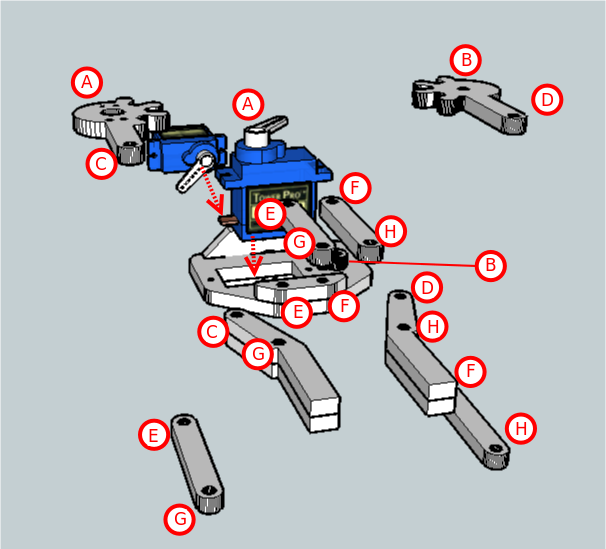
\includegraphics[scale=0.7]{images/Assembly/1-2.png}
			\caption{Assembly of the gripper }
			\label{ass1}
	\end{figure}
	\bigskip

The end result can be seen in Figure \ref{ass2}, which can also be used for reference during assembly.\\


	\begin{figure}[H]
			\centering
			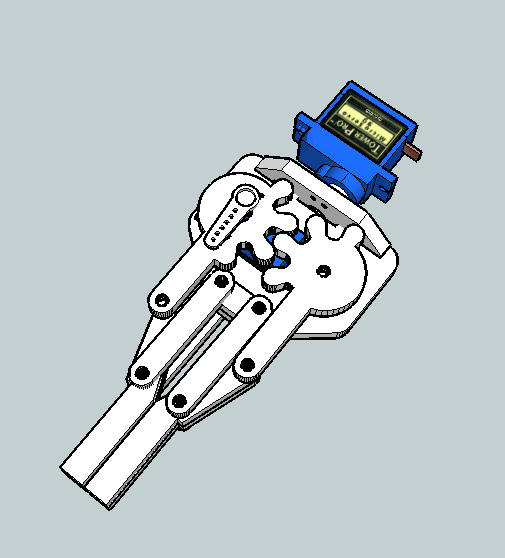
\includegraphics[scale=0.4]{images/Assembly/2.png}
			\caption{Detail of the gripper assembled}
			\label{ass2}
	\end{figure}
	\bigskip

The next step is to attach the forearm to the gripper. This is done by snapping the wrist servo into its socket and securing it in place with screws.\\

	\begin{figure}[H]
			\centering
			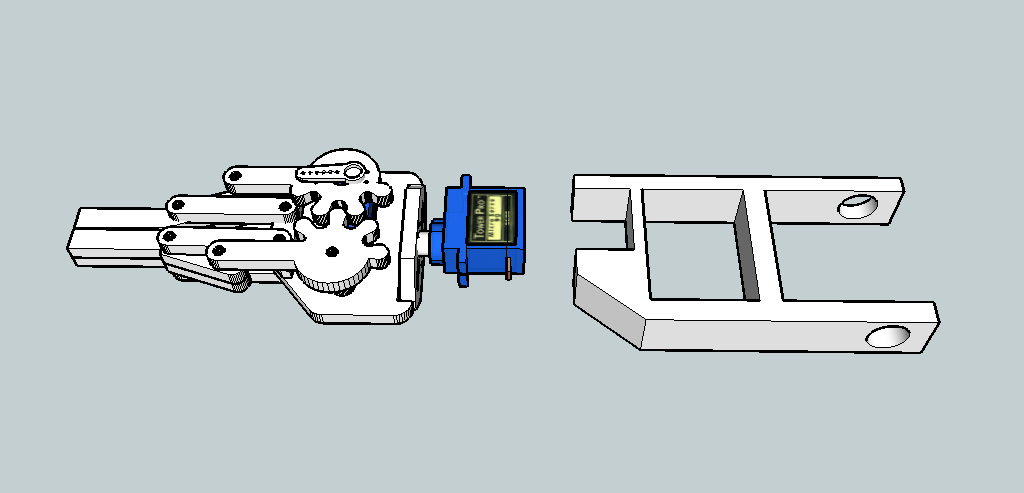
\includegraphics[scale=0.45]{images/Assembly/3.png}
			\caption{Connection of the gripper to the forearm }
			\label{ass3}
	\end{figure}
	\bigskip

Once the gripper and forearm are attached, the elbow needs to be assembled (Figure \ref{ass5}). This is done by introducing one of the Goteck servos through the hole and screwing a shafted lid designed by (obijuan) .\\


	% \begin{figure}[H]
	% 		\centering
	% 		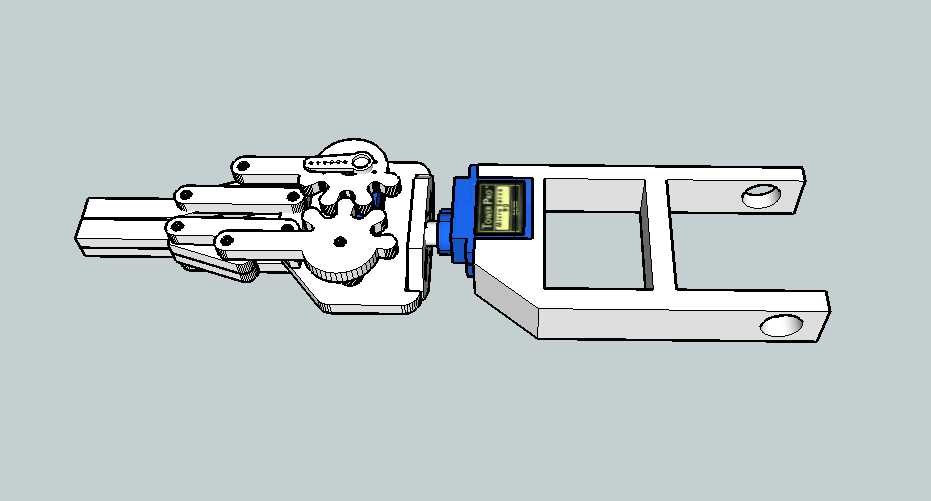
\includegraphics[scale=0.5]{images/Assembly/4.png}
	% 		\caption{Electrical connections diagram }
	% 		\label{ass4}
	% \end{figure}
	% \bigskip




	\begin{figure}[H]
			\centering
			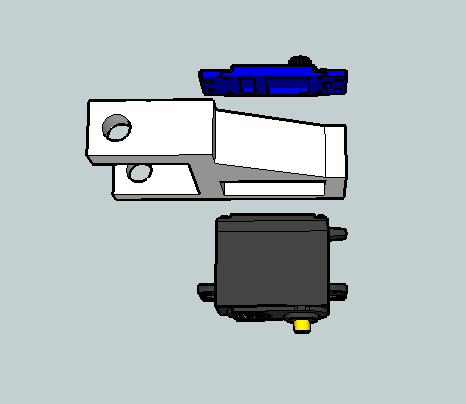
\includegraphics[scale=0.5]{images/Assembly/5.png}
			\caption{Detail of elbow assembly}
			\label{ass5}
	\end{figure}
	\bigskip




	% \begin{figure}[H]
	% 		\centering
	% 		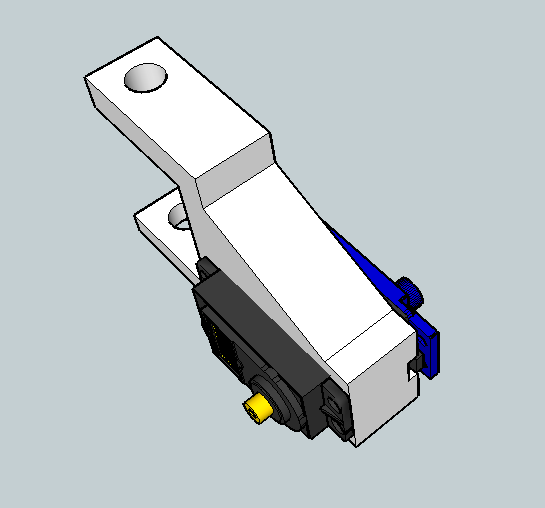
\includegraphics[scale=0.5]{images/Assembly/6.png}
	% 		\caption{Electrical connections diagram }
	% 		\label{ass6}
	% \end{figure}
	% \bigskip


Figure \ref{ass7} shows how the elbow is snapped into the rear of the forearm, by bending slightly the latter's prongs.\\

	\begin{figure}[H]
			\centering
			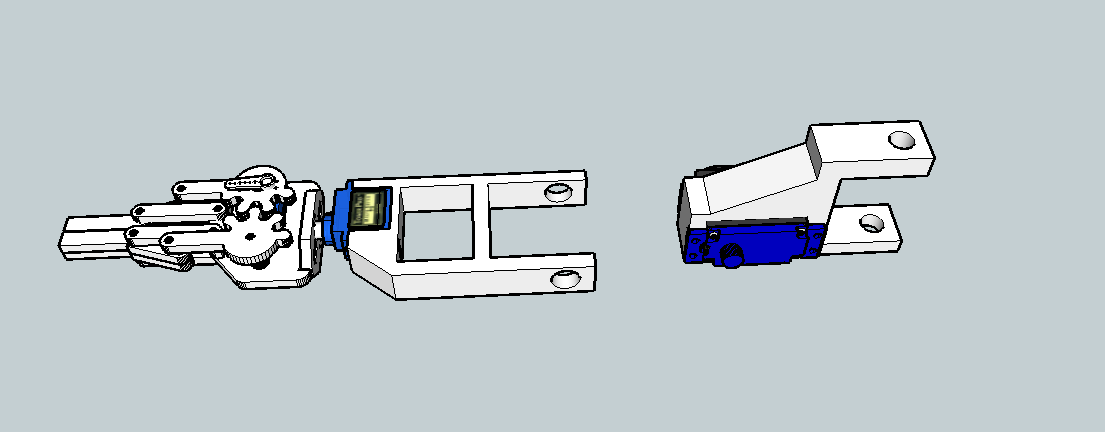
\includegraphics[scale=0.5]{images/Assembly/7.png}
			\caption{Linkage of the elbow to the forearm }
			\label{ass7}
	\end{figure}
	\bigskip





	% \begin{figure}[H]
	% 		\centering
	% 		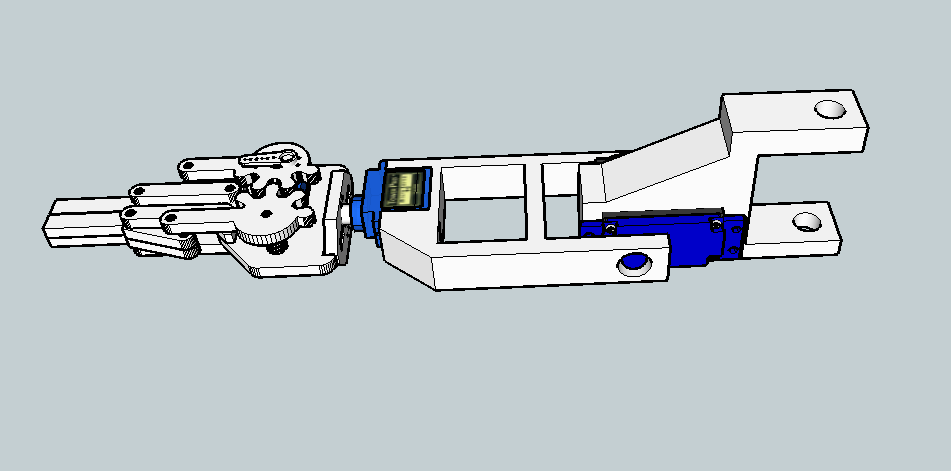
\includegraphics[scale=0.5]{images/Assembly/8.png}
	% 		\caption{Electrical connections diagram }
	% 		\label{ass8}
	% \end{figure}
	% \bigskip


The upper arm module is fitted with a Futaba servo in the same fashion as the elbow (Figure \ref{ass9}) and then fitted into the elbow piece in the same manner as the previous unit (Figure \ref{ass11}).\\

	\begin{figure}[H]
			\centering
			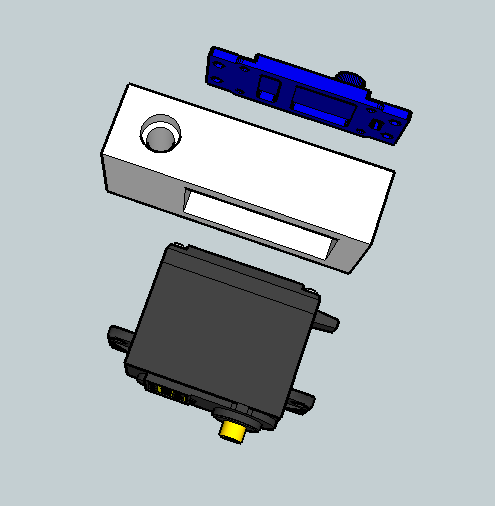
\includegraphics[scale=0.5]{images/Assembly/9.png}
			\caption{Detail of upper arm assembly }
			\label{ass9}
	\end{figure}
	\bigskip





	% \begin{figure}[H]
	% 		\centering
	% 		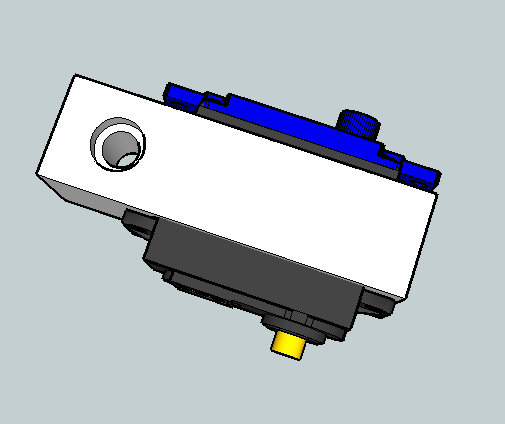
\includegraphics[scale=0.5]{images/Assembly/10.png}
	% 		\caption{Electrical connections diagram }
	% 		\label{ass10}
	% \end{figure}
	% \bigskip





	\begin{figure}[H]
			\centering
			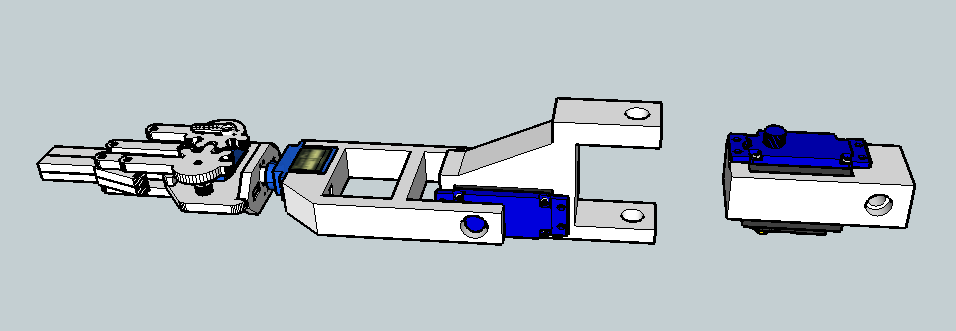
\includegraphics[scale=0.5]{images/Assembly/11.png}
			\caption{Coupling of the upper arm to the elbow }
			\label{ass11}
	\end{figure}
	\bigskip





	% \begin{figure}[H]
	% 		\centering
	% 		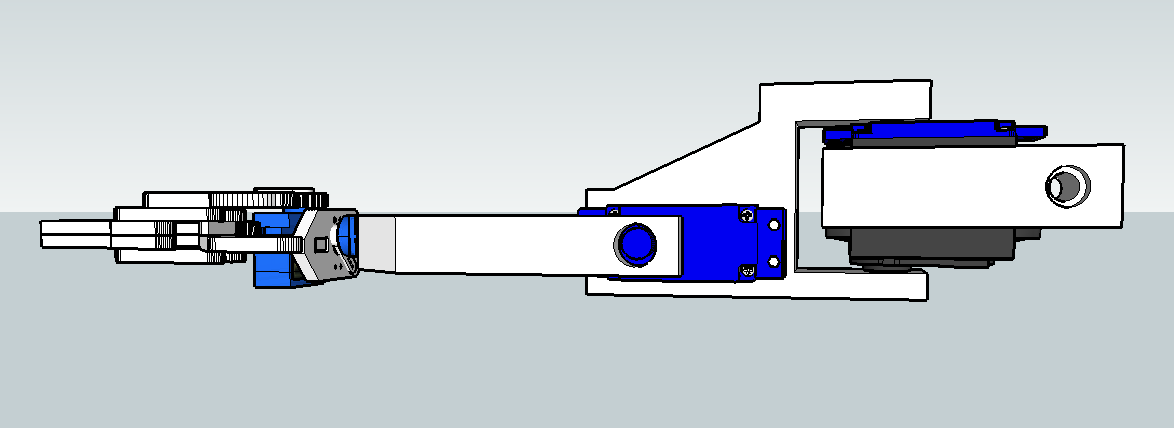
\includegraphics[scale=0.5]{images/Assembly/12.png}
	% 		\caption{Electrical connections diagram }
	% 		\label{ass12}
	% \end{figure}
	% \bigskip

Next, two 623ZZ bearings are placed each into the upper arm (Figure \ref{ass13}) and shoulder (Figure \ref{ass15}) modules. The latter also has a Goteck
servo inserted in place.\\

	\begin{figure}[H]
			\centering
			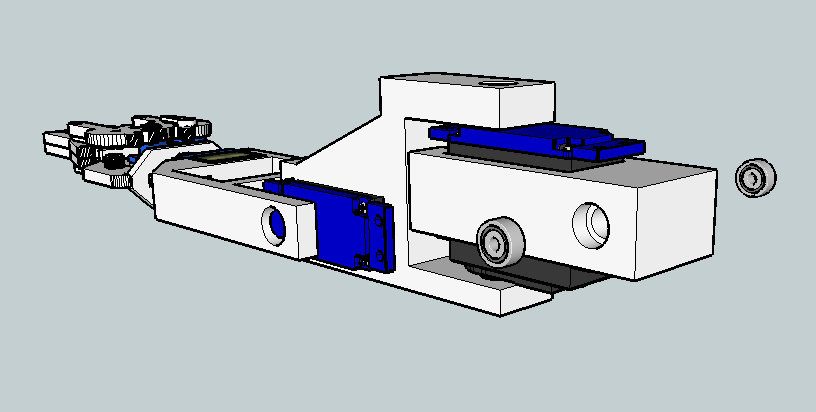
\includegraphics[scale=0.5]{images/Assembly/13.png}
			\caption{Detail of bearings insertion into the upper arm }
			\label{ass13}
	\end{figure}
	\bigskip



	% \begin{figure}[H]
	% 		\centering
	% 		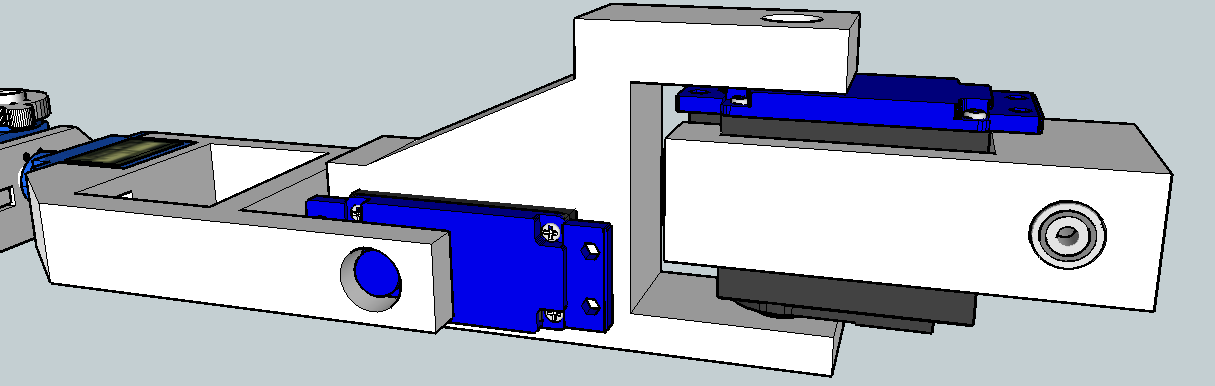
\includegraphics[scale=0.5]{images/Assembly/14.png}
	% 		\caption{Electrical connections diagram }
	% 		\label{ass14}
	% \end{figure}
	% \bigskip


	\begin{figure}[H]
			\centering
			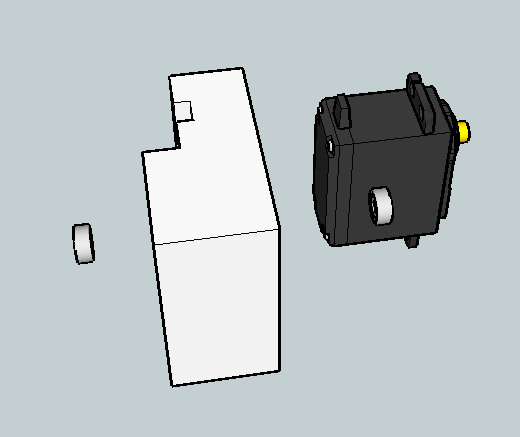
\includegraphics[scale=0.5]{images/Assembly/15.png}
			\caption{Detail of shoulder assembly }
			\label{ass15}
	\end{figure}
	\bigskip


	% \begin{figure}[H]
	% 		\centering
	% 		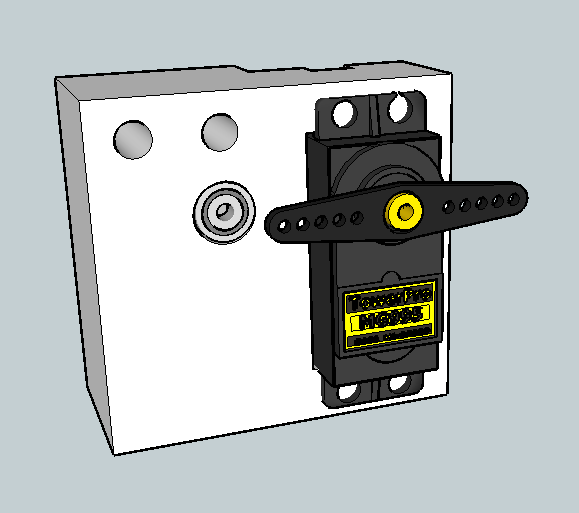
\includegraphics[scale=0.5]{images/Assembly/16.png}
	% 		\caption{Electrical connections diagram }
	% 		\label{ass16}
	% \end{figure}
	% \bigskip

The completed arm is linked to the shoulder part through a M3x120mm threaded rod and secured in place with four M3 nuts, which will avoid lateral displacement  (Figure \ref{ass17}). This is done to discharge the servomotor from the arm's weight, so it only needs to provide torque for turning, but not have to support the load.\\

	\begin{figure}[H]
			\centering
			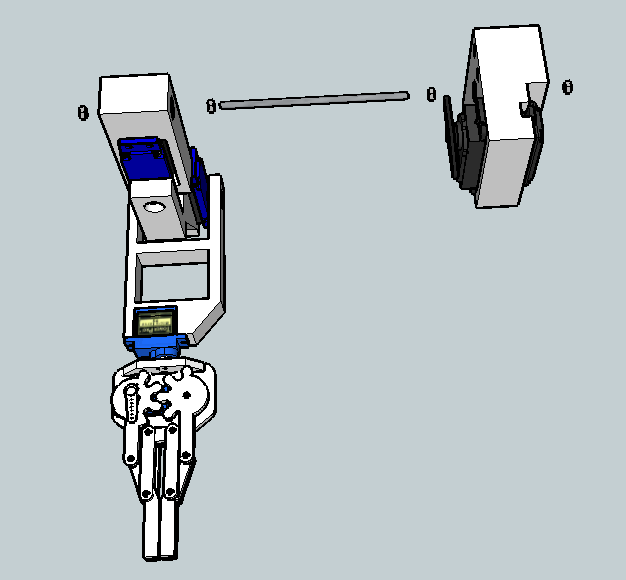
\includegraphics[scale=0.5]{images/Assembly/17.png}
			\caption{Coupling between arm and shoulder }
			\label{ass17}
	\end{figure}
	\bigskip

Figure \ref{ass19} shows the mechanical linkage between the servo and the upper arm module, which is able to rotate freely at both ends, providing traction to move the arm around the shoulder axis.\\

	\begin{figure}[H]
			\centering
			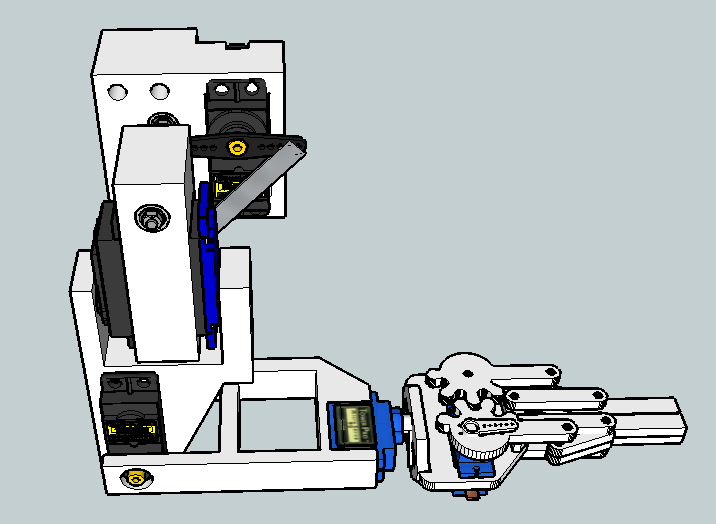
\includegraphics[scale=0.5]{images/Assembly/19.png}
			\caption{Detail of linkage between the shoulder servo and the upper arm}
			\label{ass19}
	\end{figure}
	\bigskip

	
Figures \ref{ass31} and \ref{ass32} show how the Raspberry Pi and the webcam are secured to the robot's head with two stripes of 20x80mm velcro for the former and one stripe of 20x40mm velcro for the latter.\\



	\begin{minipage}{\linewidth}
      \centering
      \begin{minipage}{0.45\linewidth}
          \begin{figure}[H]
            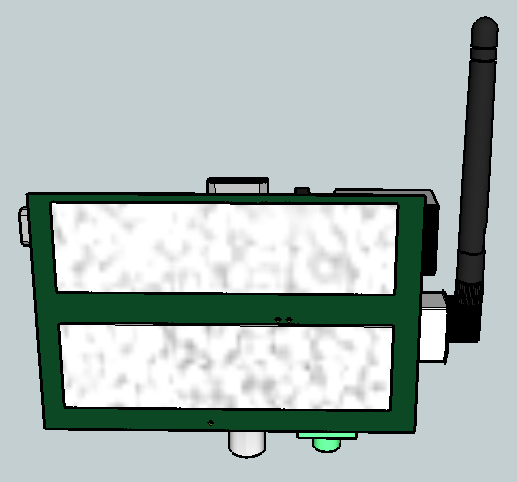
\includegraphics[scale=0.35]{images/Assembly/31.png}
			\caption{Detail of velcro stripes used to secure the Raspberry Pi }
			\label{ass31}
          \end{figure}
      \end{minipage}
      \hspace{0.05\linewidth}
      \begin{minipage}{0.45\linewidth}
          \begin{figure}[H]
              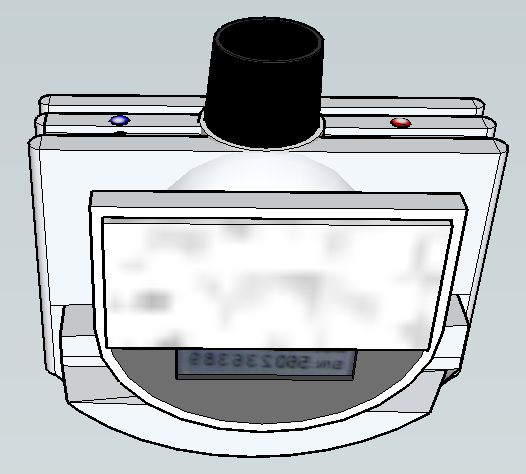
\includegraphics[scale=0.35]{images/Assembly/32.png}
			\caption{Detail of velcro stripe used to secure the camera}
			\label{ass32}
          \end{figure}
      \end{minipage}
  \end{minipage}
	\bigskip	


Similarly, both the Raspberry and the camera are attached to the head module through yet another set of two 20x80mm and one 20x40mm stripes of velcro, as seen in Figure \ref{ass33}.\\


	\bigskip
	\begin{figure}[H]
			\centering
			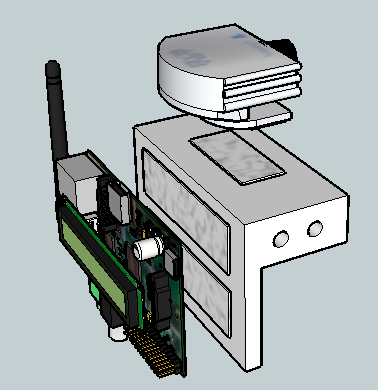
\includegraphics[scale=0.7]{images/Assembly/33.png}
			\caption{Coupling of the electronics to the robot's head }
			\label{ass33}
	\end{figure}
	\bigskip

\newpage
The procedure is repeated for the other arm, and both of these together with the head are fastened via two M5x250mm threaded rods and a set of six M5 nuts per rod to hold the different modules in position relative to each other (Figure \ref{ass22}).\\

	\begin{figure}[H]
			\centering
			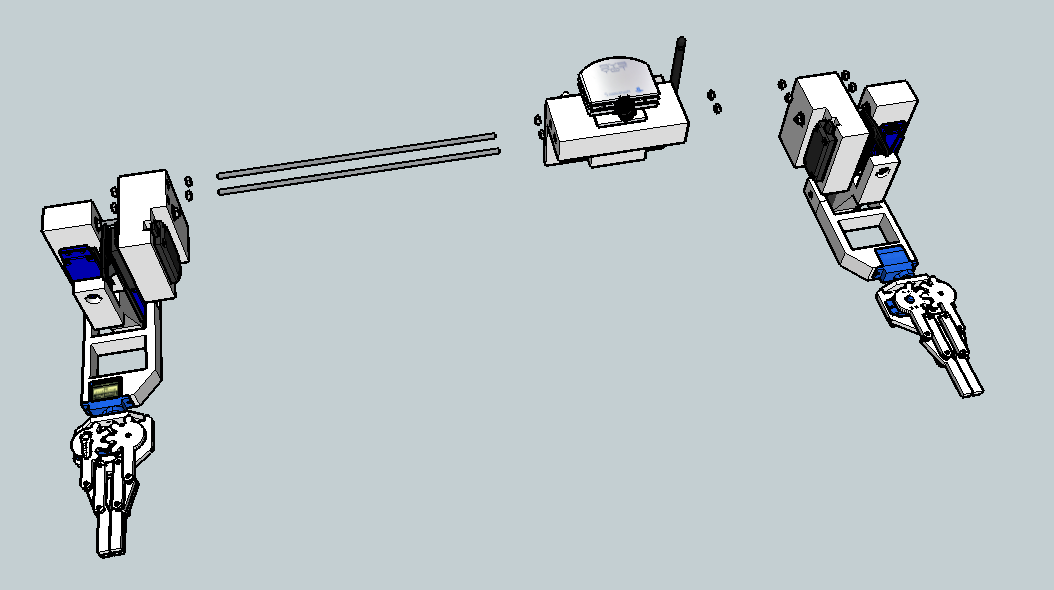
\includegraphics[scale=0.4]{images/Assembly/20.png}
			\caption{Assembly of the upper body }
			\label{ass22}
	\end{figure}
	\bigskip

	% \begin{figure}[H]
	% 		\centering
	% 		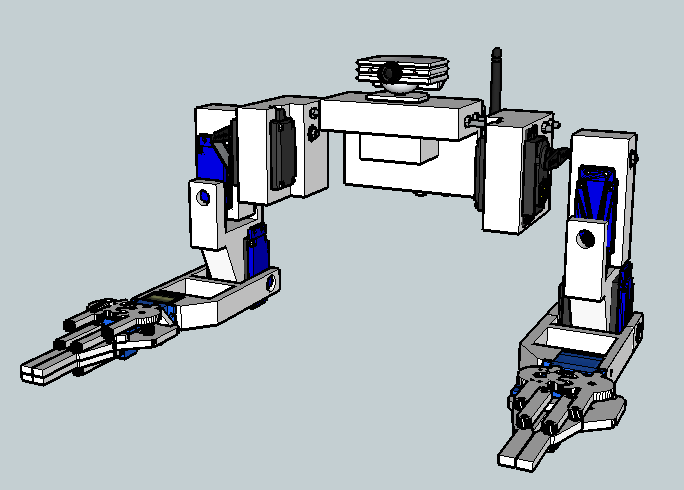
\includegraphics[scale=0.5]{images/Assembly/21.png}
	% 		\caption{Electrical connections diagram }
	% 		\label{ass21}
	% \end{figure}
	% \bigskip

As shown in Figure \ref{ass22}, the upper body is kept in positon by three pairs of rods, which prevent the  body from tilting on either side nor falling forwards due to the arm's torque. The lateral rods are M5x220mm while the central ones measure 250mm while also being M5.\\

	\begin{figure}[H]
			\centering
			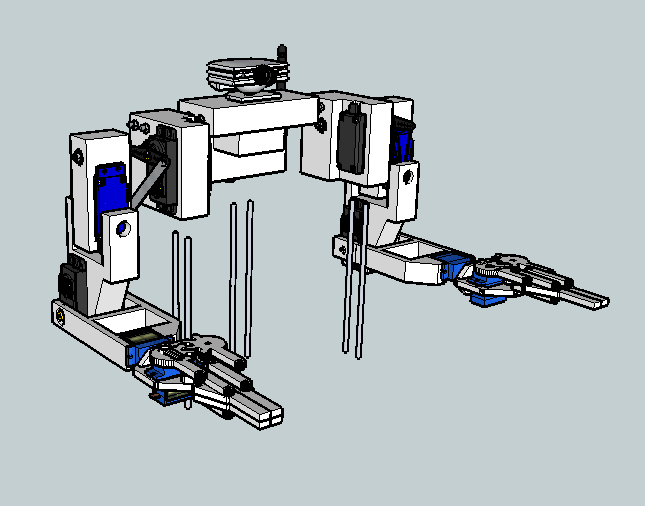
\includegraphics[scale=0.45]{images/Assembly/22.png}
			\caption{Detail of support rods insertion }
			\label{ass22}
	\end{figure}
	\bigskip


	% \begin{figure}[H]
	% 		\centering
	% 		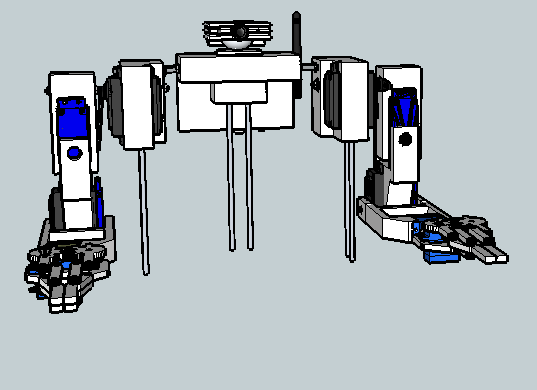
\includegraphics[scale=0.5]{images/Assembly/23.png}
	% 		\caption{Electrical connections diagram }
	% 		\label{ass23}
	% \end{figure}
	% \bigskip

The robot base consists of a 200x200x30mm wooden plank, chosen due to its resistance and as a faster and cheaper solution for a plane than a 3D printed part. The two motors are snapped into the wheels and fastened to the plank with zip ties while the caster wheel is screwed with four self-tapping screws (Figure \ref{ass24}).\\

	\begin{figure}[H]
			\centering
			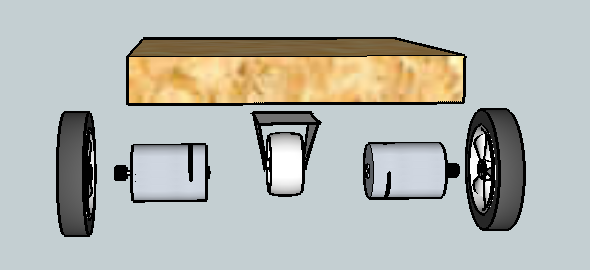
\includegraphics[scale=0.5]{images/Assembly/24.png}
			\caption{Detail of base assebly  }
			\label{ass24}
	\end{figure}
	\bigskip




	% \begin{figure}[H]
	% 		\centering
	% 		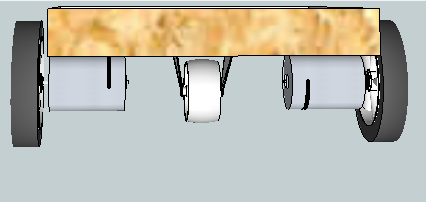
\includegraphics[scale=0.5]{images/Assembly/25.png}
	% 		\caption{Electrical connections diagram }
	% 		\label{ass25}
	% \end{figure}
	% \bigskip

The upper body and the base are then joined together as illustrated by Figure \ref{ass26}, by inserting M5 nuts at either side of each of the base throughout the rods.\\

	\begin{figure}[H]
			\centering
			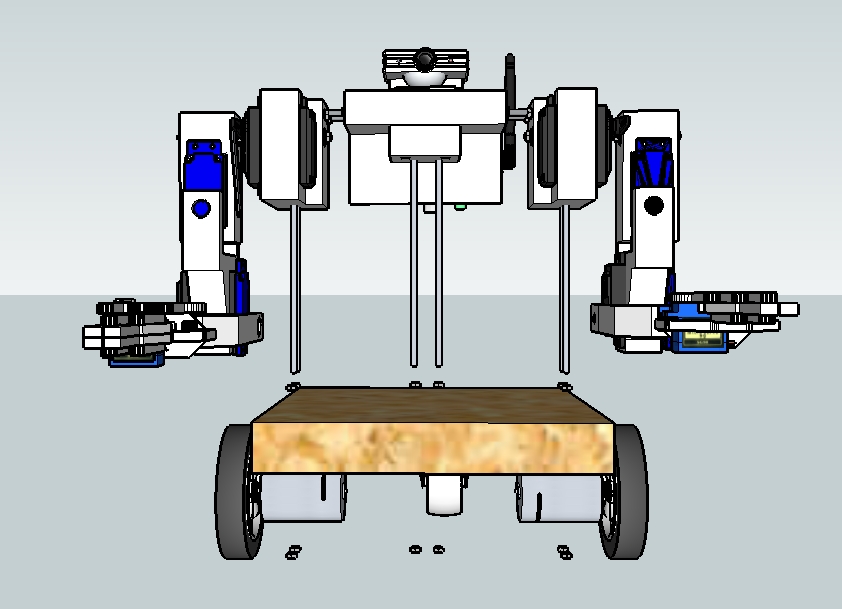
\includegraphics[scale=0.5]{images/Assembly/26.png}
			\caption{Connection of upper body to base }
			\label{ass26}
	\end{figure}
	\bigskip



	% \begin{figure}[H]
	% 		\centering
	% 		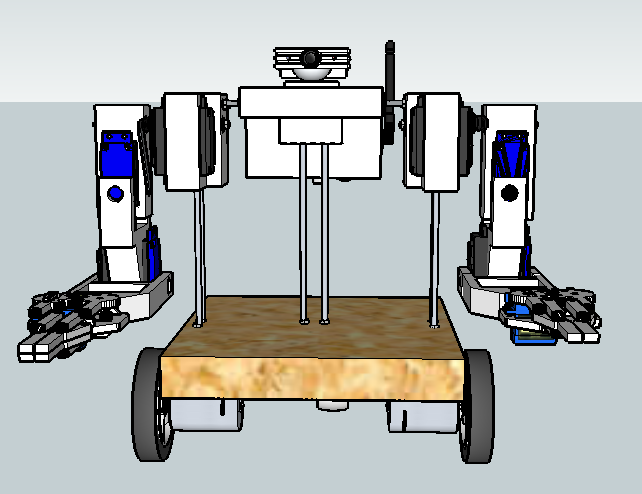
\includegraphics[scale=0.5]{images/Assembly/27.png}
	% 		\caption{Electrical connections diagram }
	% 		\label{ass27}
	% \end{figure}
	% \bigskip
 \newpage
 Figure \ref{ass28} exhibits the disposition of two more 20x180mm velcro stripes intended to secure in place both the battery and the circuit board containing the Arduino, level converters and motor driver. \\

	\begin{figure}[H]
			\centering
			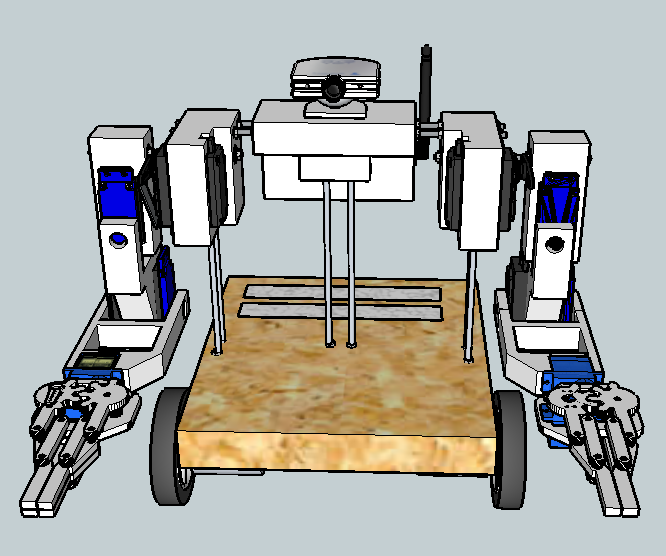
\includegraphics[scale=0.5]{images/Assembly/28.png}
			\caption{Detail of velcro stripes in the base}
			\label{ass28}
	\end{figure}
	\bigskip

Figure \ref{ass29} presents the velcro stripes at the bottom of the battery and circuit board. These are 20x100mm in dimension and are to be connected to the ones on the base of the bot.\\

	\begin{figure}[H]
			\centering
			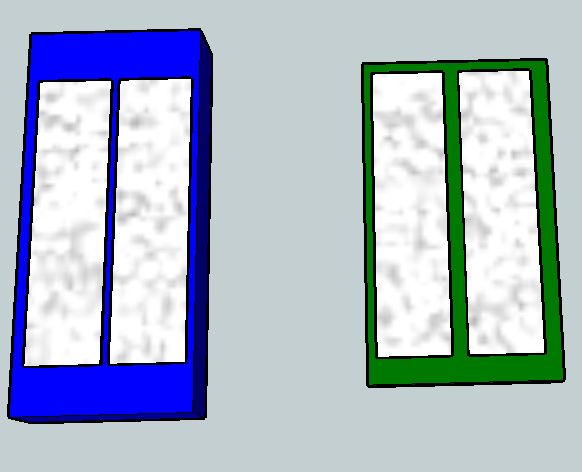
\includegraphics[scale=0.3]{images/Assembly/29.png}
			\caption{Detail of velcro stripes in the battery(L) and circuit board(R) }
			\label{ass29}
	\end{figure}
	\bigskip

\newpage
Finally, Figure \ref{ass30} shows the robot fully assembled and in resting position.\\

	\begin{figure}[H]
			\centering
			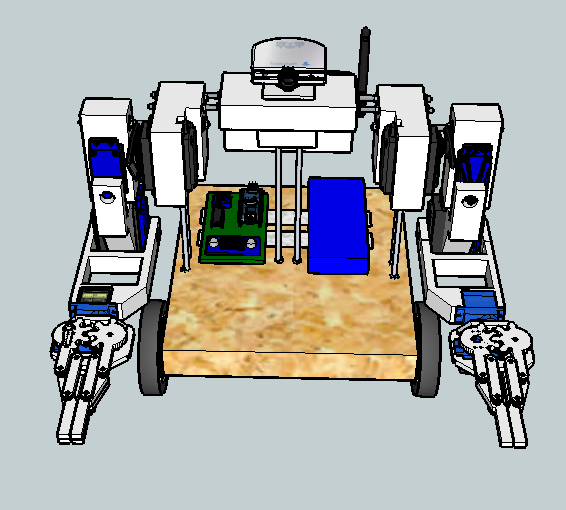
\includegraphics[scale=0.5]{images/Assembly/30.png}
			\caption{Assembled robot }
			\label{ass30}
	\end{figure}
	\bigskip


Figure \ref{ass31} lists all of the robot's actuators for later identification, classifying them into servomotors (S) or motors (M) and left(L) and right (R) sides.\\

\begin{figure}[H]
			\centering
			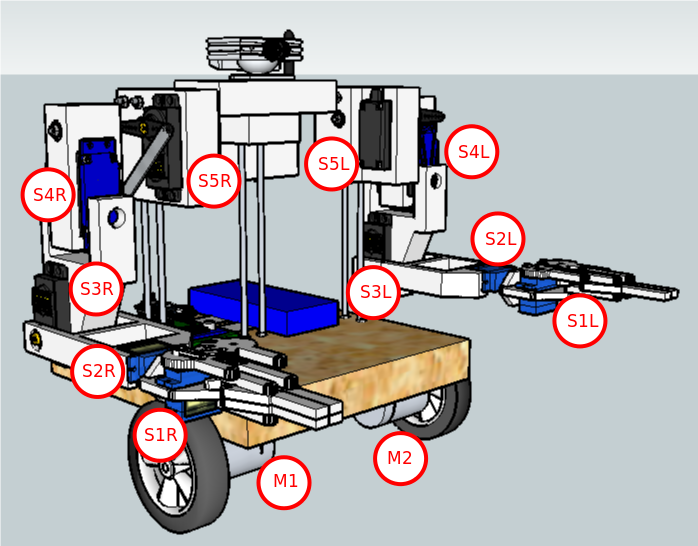
\includegraphics[scale=0.45]{images/Assembly/34-2.png}
			\caption{Detail of the robot's actuators }
			\label{ass31}
	\end{figure}
	\bigskip


















































































\subsection{Connections}

This section will present how the different elements composing the robot are connected, first from the electrical point of view, then from a means of communication angle and finally from the different programs' interactions perspective.



%%%%%%%%%% ELECTRIC %%%%%%%%%%%%%%%%%%%%%%%%%%%%%%%%%%%%%%%%%%%%%%%%%%%%%%%

\subsubsection{Electrical connections}

Figure \ref{electricDiagram} shows how the different electric and electronic components are interconnected.  As it can be seen, different voltage levels co-exist within the robot, so regulators are placed to ensure the components function correctly. \\

The DC motors need the highest voltage to work, and so are connected to the battery, which provides them with the 12V they need. However they have to be controlled by the Arduino, hence the need for a driver that will turn on and off the 12V rails from 5V signals.\\

The rest of the components operate at 5V, which is why the step-down converter is used to convert the battery's 12V output into the desired level. The Raspberry Pi, Arduino and servomotors are connected to this rail.\\

Finally, the Raspberry communicates with the Arduino through the former's UART pins, which operate at a 3.3V level and can be damaged by the latter's 5V level pins. To avoid this a logic level shifter is introduced, which ensures data transmission without compromising the hardware's integrity.\\

	\begin{figure}[H]
			\centering
			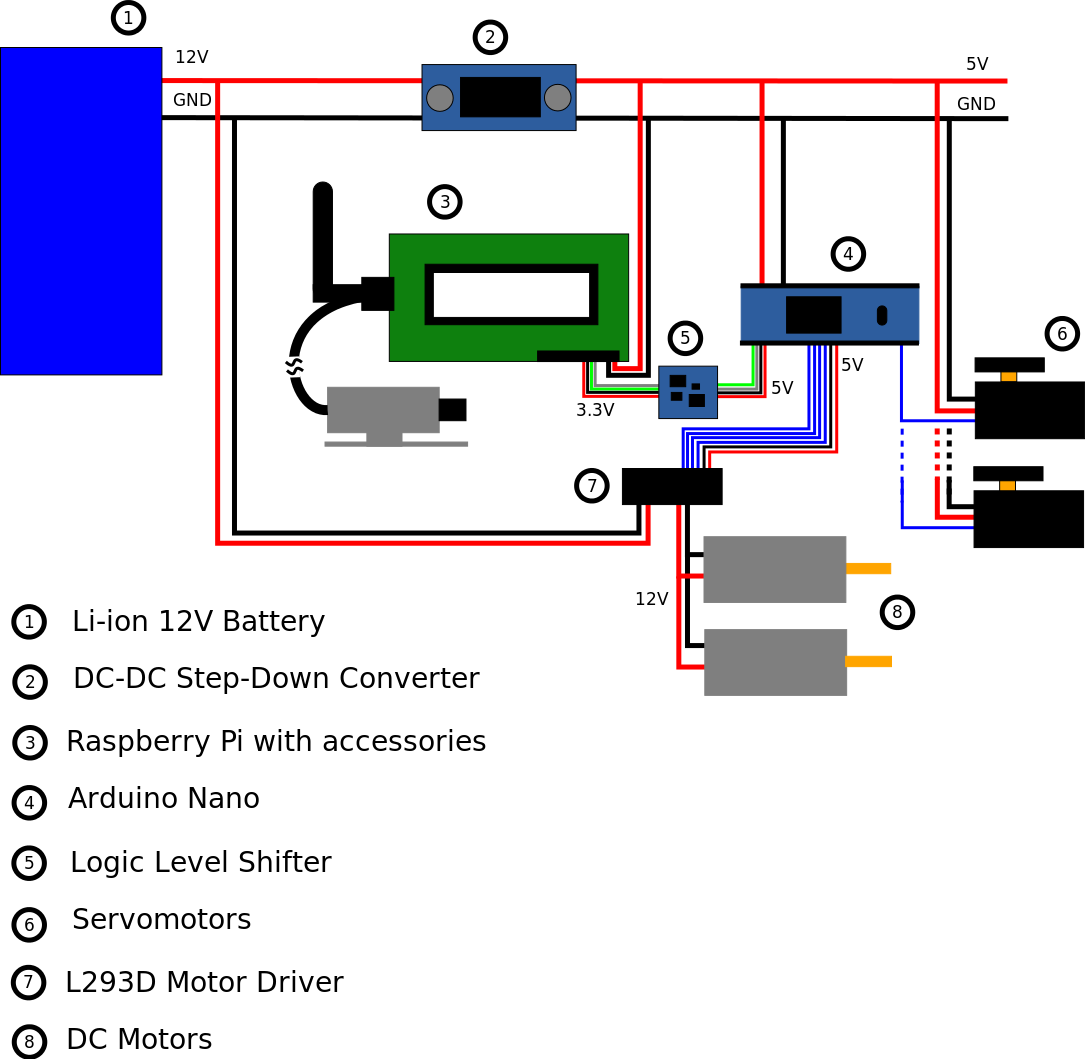
\includegraphics[width=15cm, angle=0]{images/Diagrams/electrical.png}
			\caption{Electrical connections diagram }
			\label{electricDiagram}
	\end{figure}
	\bigskip
	
\bigskip


The previous diagram shows how all components are interconnected, but to increase its clarity some connections have not been shown in detail. The following diagrams show how the remaining elements are wired pin by pin.

	\begin{itemize}
	\item Figure \ref{gpioDetail} shows the conections between the LCD and Rasbperry Pi and the Raspberry, Arduino and the logic voltage shifter pins.
	\end{itemize}

	\begin{figure}[H]
			\centering
			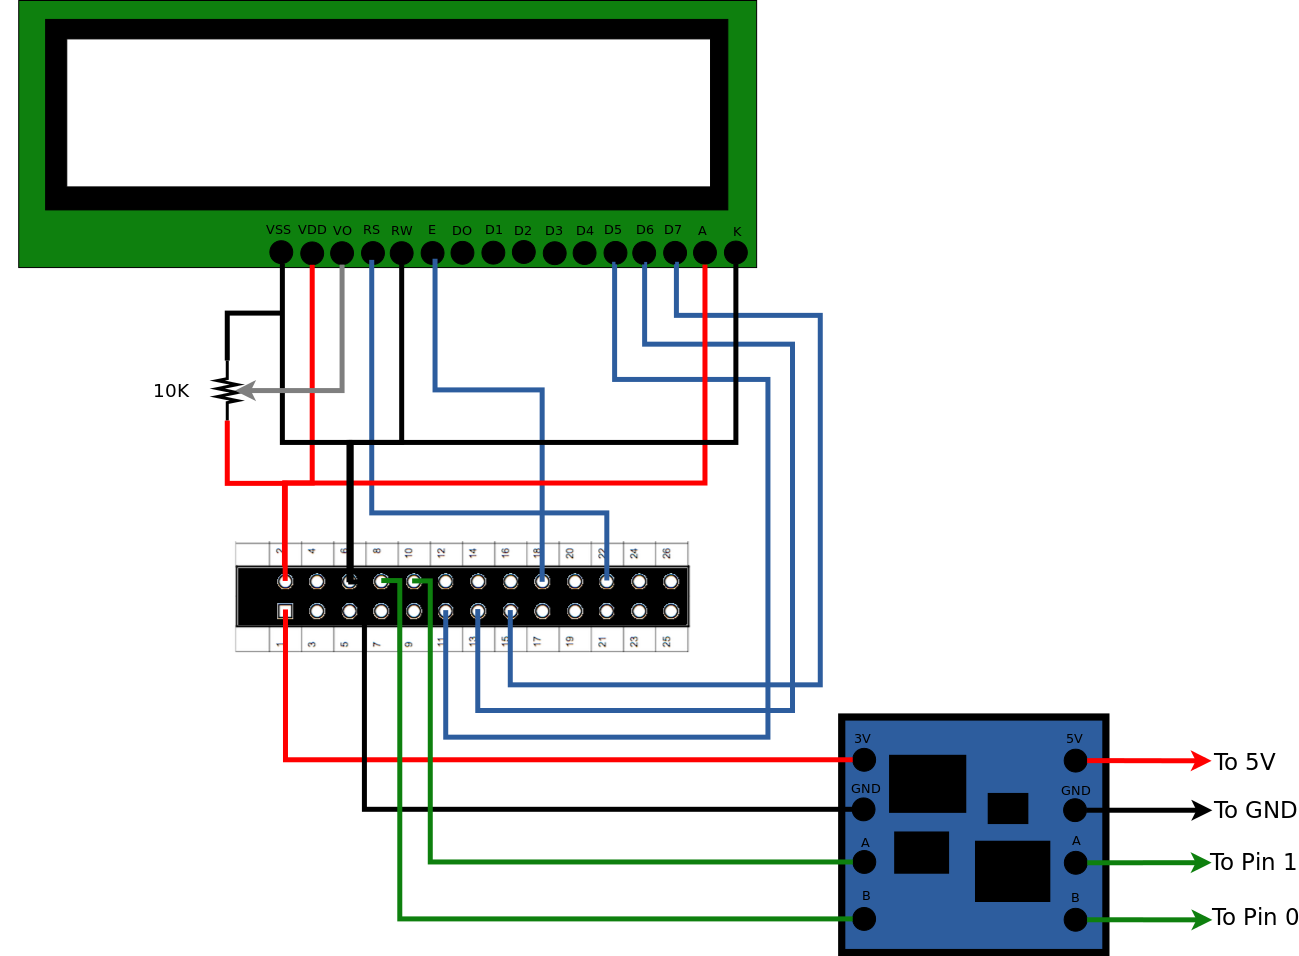
\includegraphics[width=15cm, angle=0]{images/Diagrams/detail.png}
			\caption{Detail of LCD and Serial connections }
			\label{gpioDetail}
	\end{figure}
	\bigskip


	\bigskip
	\begin{itemize}
	\item Figure \ref{hbridgeDetail} shows the wiring between the motor driver, the motors and the Arduino.
	\end{itemize}
	
	\begin{figure}[H]
			\centering
			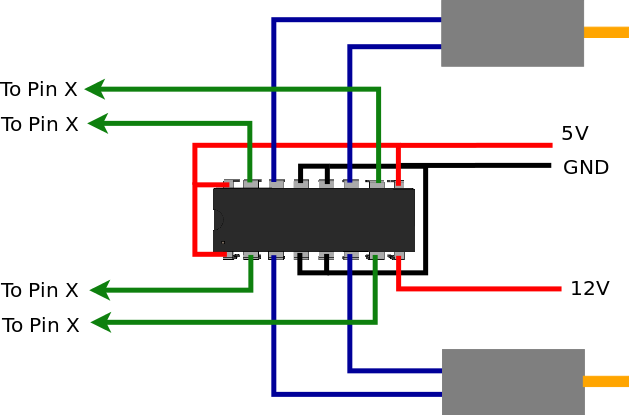
\includegraphics[scale=0.5, angle=0]{images/Diagrams/hbridge.png}
			\caption{Detail of motor driver wiring }
			\label{hbridgeDetail}
	\end{figure}
	\bigskip

	\begin{itemize}
	\item Figure X shows which element is connected to each of the Arduino pins

	\item "table with servo +motor letters assigned to arduino pins"
	\end{itemize}


%%%%%%%%%% LOGIC %%%%%%%%%%%%%%%%%%%%%%%%%%%%%%%%%%%%%%%%%%%%%%%%%%%%%%%

\subsubsection{Logic connections}

Figure \ref{logicDiagram} shows how the different components communicate between themselves. As it can be seen, the user controls the robot from the Android application. This implements a bidirectional communication over wifi with the Raspberry Pi, which is used to both send the Raspberry data concerning the movement of the different motors and to receive the video stream from the robot's onboard camera. The Raspberry then communicates over Serial port with the Arduino, which takes care of the data received to obey the user's commands.\\

	\begin{figure}[H]
			\centering
			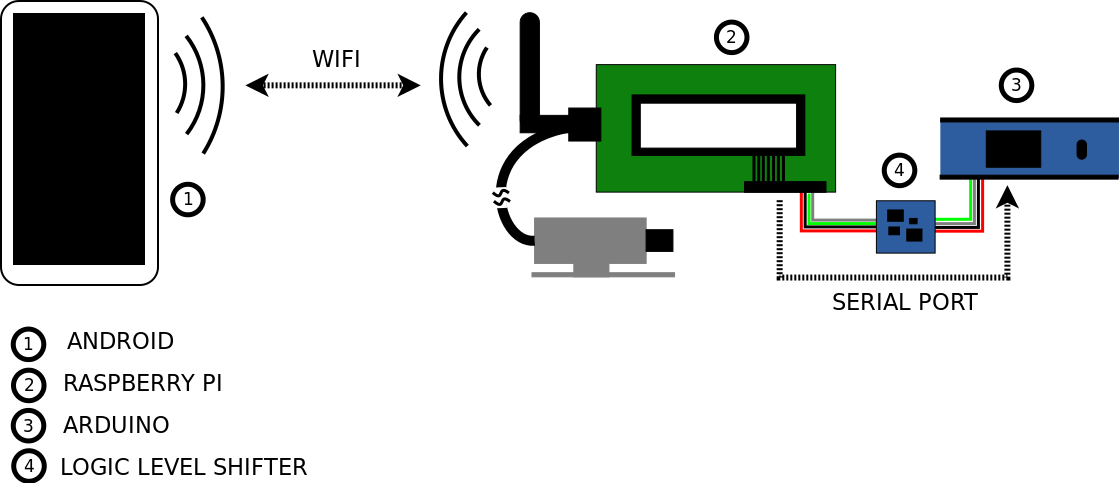
\includegraphics[width=15cm, angle=0]{images/Diagrams/logic.png}
			\caption{Logic connections diagram }
			\label{logicDiagram}
	\end{figure}
	\bigskip

%%%%%%%%%% SW %%%%%%%%%%%%%%%%%%%%%%%%%%%%%%%%%%%%%%%%%%%%%%%%%%%%%%%

\subsubsection{Software connections}

Figure \ref{swDiagram} shows how the different programs interconnect the various components. It can thus be seen that the Raspberry Pi will first create a wifi network and then start to stream video through it. The android phone on the other hand will connect itself to the recently created network and will use it to emit the commands given by the user. The Raspberry will have already started the IP/UART Bridge, and will send the data received from the phone to the Arduino. Finally, the latter will execute its code to execute the orders received.\\

	\begin{figure}[H]
			\centering
			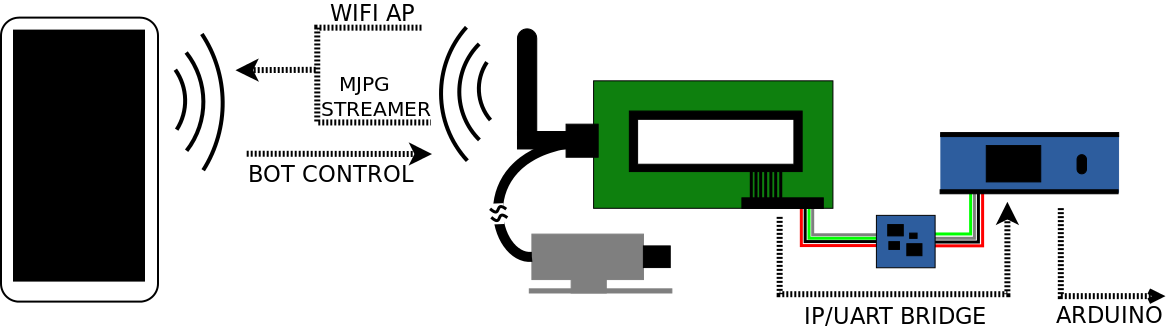
\includegraphics[width=15cm, angle=0]{images/Diagrams/software.png}
			\caption{Software connections diagram }
			\label{swDiagram}
	\end{figure}
	\bigskip

